\chapter{Event Selection}
\label{chapter:event_selection}

This chapter defines the signal regions (SRs) targeting the processes shown in Figure~\ref{fig:u1_taunu_target_topologies}.
The analysis variables and preselection are introduced first, followed by the optimisation of the one-$b$-jet regions, the definition of the zero-$b$-jet regions, and a study of $\tau\tau$ signal contamination in the SRs.

\section{Preselection and variables definition}
\label{sec:ch7_preselection}

\subsection{Analysis variables}
\label{subsec:ch7_variables}

The transverse mass $\mT$ of the $\tau$ and $\mpt$ system is defined as
    \begin{equation}
        \mT = \sqrt{2\pT^\tau\met\left[1-\cos\DphiTauMet\right]}.
        \label{eq:ch7_mt}
    \end{equation}
Here $\DphiTauMet$ is the separation in $\phi$ between the $\tau$ momentum and $\mpt$.
The variable $\mT$ is used to probe the high-energy tail of the $\tau\nu$ final state, which is particularly sensitive to non-resonant leptoquark contributions~\cite{Endo2022NonResonant}.

The invariant masses $m_{b\tau}$ and $m_{j\tau}$ are defined as:
    \begin{equation}
        m_{b\tau}^{2} = (p_b+p_\tau)^2, \qquad m_{j\tau}^{2} = (p_{j_1}+p_\tau)^2,
        \label{eq:ch7_visible_masses}
    \end{equation}
    where $p_b$, $p_{j_1}$ and $p_\tau$ are four-momenta, and $j_1$ is the jet with the largest $\pT$.
The zero-$b$-jet regions contain no $b$-tagged jet, so $m_{j\tau}$ is used in place of $m_{b\tau}$.

\subsection{Multijet suppression and Preselection}
\label{subsec:ch7_multijet}

Although the high $\met$ threshold rejects most multijet events, some can still enter the SRs and CRs due to the large multijet cross section. These events typically contain a misidentified $\tau$ and fake $\met$ from poor jet resolution. Therefore, further suppression is necessary.

Specifically, fake $\met$ is produced when an energetic jet is mismeasured. In this case, $\mpt$ points approximately towards that jet and it tends to be small compared with the $\pT$ of the mismeasured jet. On the other hand, in signal events, $\mpt$ from neutrinos has no such tendency.
Figure~\ref{fig:ch7_fake_met} illustrates this difference. The minimum jet--$\mpt$ separation in $\phi$ and the ratio $\metOverMinDphiJetPt$ are therefore used as discriminating variables.

\begin{figure}[htpb]
    \centering
    \begin{subfigure}{0.34\linewidth}
        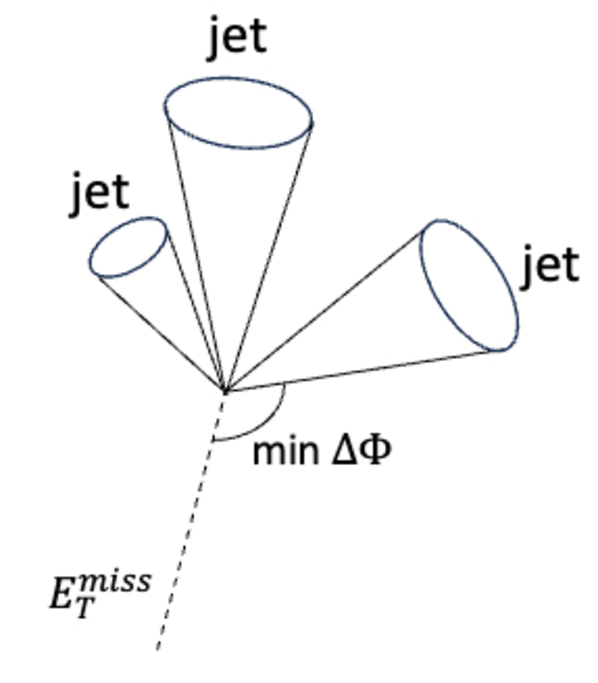
\includegraphics[width=\linewidth]{Figs/CH7/QCD/fake_met_signal.pdf}
        \caption{Signal.}
    \end{subfigure}\hspace{0.08\linewidth}
    \begin{subfigure}{0.34\linewidth}
        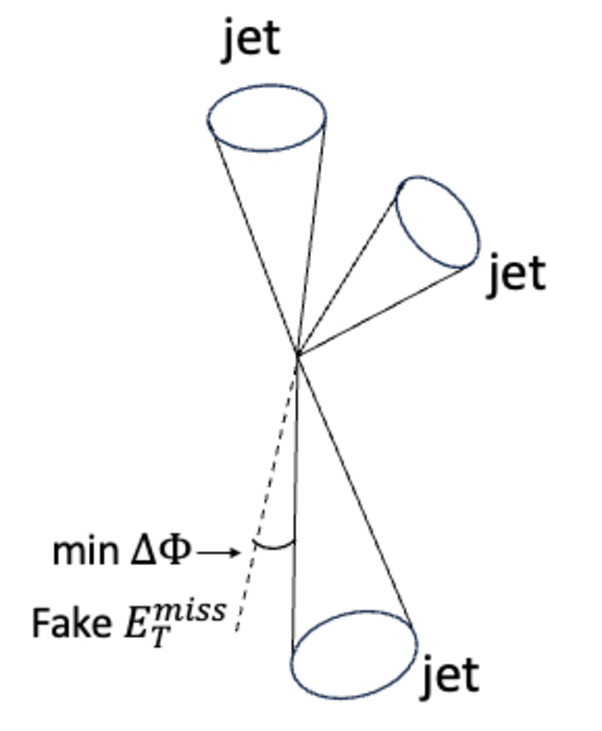
\includegraphics[width=\linewidth]{Figs/CH7/QCD/fake_met_multijets.pdf}
        \caption{Multijet background.}
    \end{subfigure}
    \caption[Missing momentum in signal and multijet events]{Schematic diagrams of (a) $\met$ from neutrinos in signal events and (b) fake $\met$ from a mismeasured energetic jet in multijet events.}
    \label{fig:ch7_fake_met}
\end{figure}
Here $\minDphiJetPt$ is the $\pT$ of the jet with the smallest $\DphiJetMet$.

Events are retained if
\begin{equation}
    \minDphiJetMet>0.4 \quad\text{or}\quad \metOverMinDphiJetPt>6.
    \label{eq:ch7_qcd_cut}
\end{equation}
The study used to determine the threshold above is presented in detail in Appendix~\ref{App:QCD_bkg_study}.

In addition to the multijet suppression requirement, the following preselection requirements are applied before the SR optimisation:
\begin{itemize}
  \item The lowest-threshold unprescaled $\met$ trigger to select events with large $\met$.
  \item $\met>200~\GeV$ for full trigger efficiency.
  \item Exactly one signal $\tau$.
  \item A signal electron/muon veto.
  \item Exactly one $b$-tagged jet for the one-$b$-jet SR ($\bTagSR$).
  \item At least one untagged jet and no $b$-tagged jets for the $b$-jet-veto SR ($\bVetoSR$).
\end{itemize}

\section[$\bTagSR$ optimisation and definition]{$\bTagSR$ optimisation and definition}
\label{sec:ch7_sr1b}

Event selection in $\bTagSR$ is optimised using a grid scan of thresholds on variables that help separate signal from background. $\bTagSR$-$\Res$ and $\bTagSR$-$\NonRes$ are optimised separately.

\subsection{Scan variables and criterion}
\label{subsec:ch7_scan}

$\pT^\tau$ and $\met$ are considered first, since energetic $\tau$ leptons and neutrinos are expected in the signal.
The $b$-jet $\pT$ is also used. An energetic $b$-jet from the leptoquark decay is expected in the resonant process, whereas the $b$-jet is typically softer in the non-resonant process. 
$\mT$ is used to distinguish non-resonant leptoquark exchange from the SM background.
A tighter $\mT$ threshold is therefore expected in $\bTagSR$-$\NonRes$ than in $\bTagSR$-$\Res$.
The invariant mass $m_{b\tau}$ is used to probe resonant $U_1\to b\tau$ decays.
$\DphiTauMet$ is used to select the back-to-back $\tau$ and $\mpt$ configuration of the non-resonant signal, which helps suppress the top-quark background.
On the other hand, in $\bTagSR$-$\Res$, small $\DphiTauMet$ are favoured due to the high $\pt^{b}$ requirement.
The jet multiplicity is used to suppress $\ttbar$ events since they tend to have more jets than the signal events.
The thresholds used for grid scan are summarised in Table~\ref{tab:ch7_scan_variables}.

\begin{table}[htbp]
    \centering
    \small
    \caption{Variable scan range for the $\bTagSR$ optimisation.}
    \label{tab:ch7_scan_variables}
    \begin{tabular}{lcc}
        \toprule
        Variable & $\bTagSR$-$\Res$ & $\bTagSR$-$\NonRes$ \\
        \midrule
        $\DphiTauMet$ & $<\{0.3,1.2,2.4,2.6,\pi\}$ & $>\{0.3,1.2,2.4,2.6\}$ \\
        $m_{b\tau}$ [$\GeV$] & $>\{0,800\}$ & N/A \\
        $\met$ [$\GeV$] & \multicolumn{2}{c}{$>\{200,250,300,350,400,500,600\}$} \\
        $\pT^\tau$ [$\GeV$] & \multicolumn{2}{c}{$>\{200,250,300,350,400,500,600\}$} \\
        $\mT$ [$\GeV$] & \multicolumn{2}{c}{$>\{100,200,300,400,500,600,700,800,900,1000\}$} \\
        $N_j-N_b$ & \multicolumn{2}{c}{$\leq\{1,2,3\}$} \\
        \bottomrule
    \end{tabular}
\end{table}

Note that only the $m_{b\tau}>0$ and $800~\GeV$ are tested here. Since the signal mass resolution is only about 50\% and very few background events are remained in the SRs, little improvement in sensitivity is expected from a finer mass threshold scan.

Different signal benchmarks are selected for each signal region. The optimisation for $\bTagSR$-$\Res$ uses $(\MU,\gU,\beta_L^{23})=(1.5~\TeV,1.5,0.6)$, where on-shell production is dominant.
For $\bTagSR$-$\NonRes$, the optimisation uses $(\MU,\gU,\beta_L^{23})=(2.5~\TeV,2.5,1.0)$, where $t$-channel exchange is dominant.
Interference is not included in the scan because its contribution is around $5$--$10\%$ in the parameter range probed by the $\bTagSR$ regions, as discussed in Appendix~\ref{app:signal_interference_study}. The selected cut combination is therefore not expected to change significantly when interference is included.

The expected sensitivity of each cut combination is evaluated using the significance $Z$, calculated as follows~\cite{ATL-PHYS-PUB-2020-025}:
\begin{equation}
    Z = \sqrt{2\left[n\ln\!\left(\frac{n(b+\sigma_b^2)}{b^2+n\sigma_b^2}\right)-\frac{b^2}{\sigma_b^2}\ln\!\left(\frac{b^2+n\sigma_b^2}{b(b+\sigma_b^2)}\right)\right]},
    \label{eq:ch7_optimisation_significance}
\end{equation}
where $s$ and $b$ are the expected signal and background event yields, $n=s+b$, and the background uncertainty is assumed to be $\sigma_b=0.3b$.

To obtain reliable results, the following two constraints are applied during the scan:
\begin{itemize}
    \item Cut combinations with $b\leq2$ are discarded.
    \item If a particular SM background (e.g. $\Wtaunu$) has a negative weighted yield, its contribution is set to zero.
\end{itemize}
The first constraint is used to avoid zero background estimates caused by limited MC statistics. It also ensures reliable estimates of the minor backgrounds. As a result, the MC statistical uncertainties are limited to 31\% in the resonant SR and 40\% in the non-resonant SR.

An example of the significance scan is shown in Figure~\ref{fig:ch7_met_with_significance}, along with $N-1$ $\met$ distributions.\footnote{For a selection with $N$ requirements, an $N-1$ distribution is obtained by removing the requirement on the plotted variable while keeping the other $N-1$ requirements. Here, the $\met$ requirement is removed.}
For each bin in the lower significance panels, $Z$ is calculated using the signal and background yields summed above the corresponding threshold. Points with $b\leq2$ are excluded from the cut choice.
The largest $Z$ is therefore obtained at $200~\GeV$ for $\bTagSR$-$\Res$ and $400~\GeV$ for $\bTagSR$-$\NonRes$. A similar procedure is applied to the other variables.

% \begin{figure}[htbp]
%     \centering
%     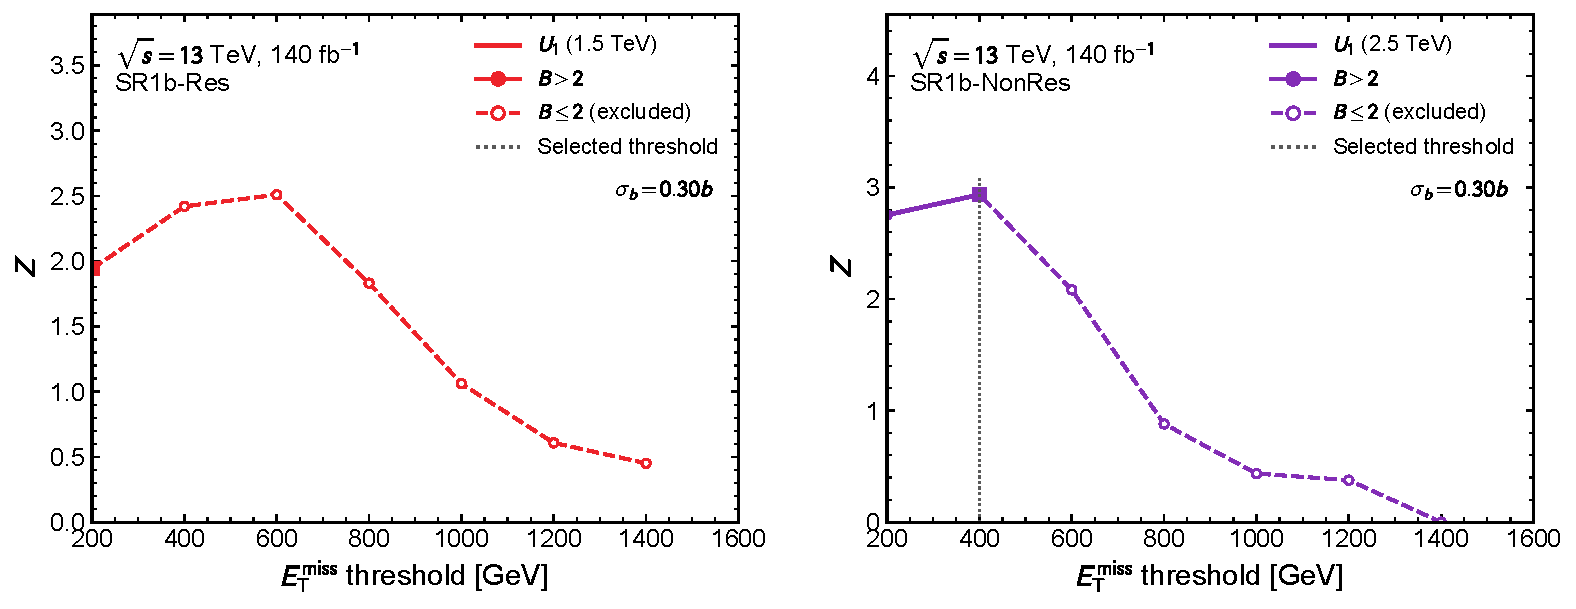
\includegraphics[width=\linewidth]{Figs/CH7/significance/SR1b_met_significance_scan.pdf}
%     \caption[SR1b significance scan in missing transverse momentum]{Approximate significance as a function of the $\met$ threshold for $\bTagSR$-$\Res$ (left) and $\bTagSR$-$\NonRes$ (right), using the pure BSM benchmarks $(\MU,\gU,\beta_L^{23})=(1.5~\TeV,1.5,0.6)$ and $(2.5~\TeV,2.5,1.0)$, respectively. The $N-1$ distributions are integrated above each threshold and Eq.~\ref{eq:ch7_optimisation_significance} is evaluated with $\sigma_b=0.30b$. Open markers and dashed segments indicate points with $b\leq2$, which are excluded from the cut choice. The selected thresholds are marked by squares and vertical dotted lines.}
%     \label{fig:ch7_met_significance_scan}
% \end{figure}

\begin{figure}[htpb]
    \centering
    \begin{subfigure}{0.8\linewidth}
        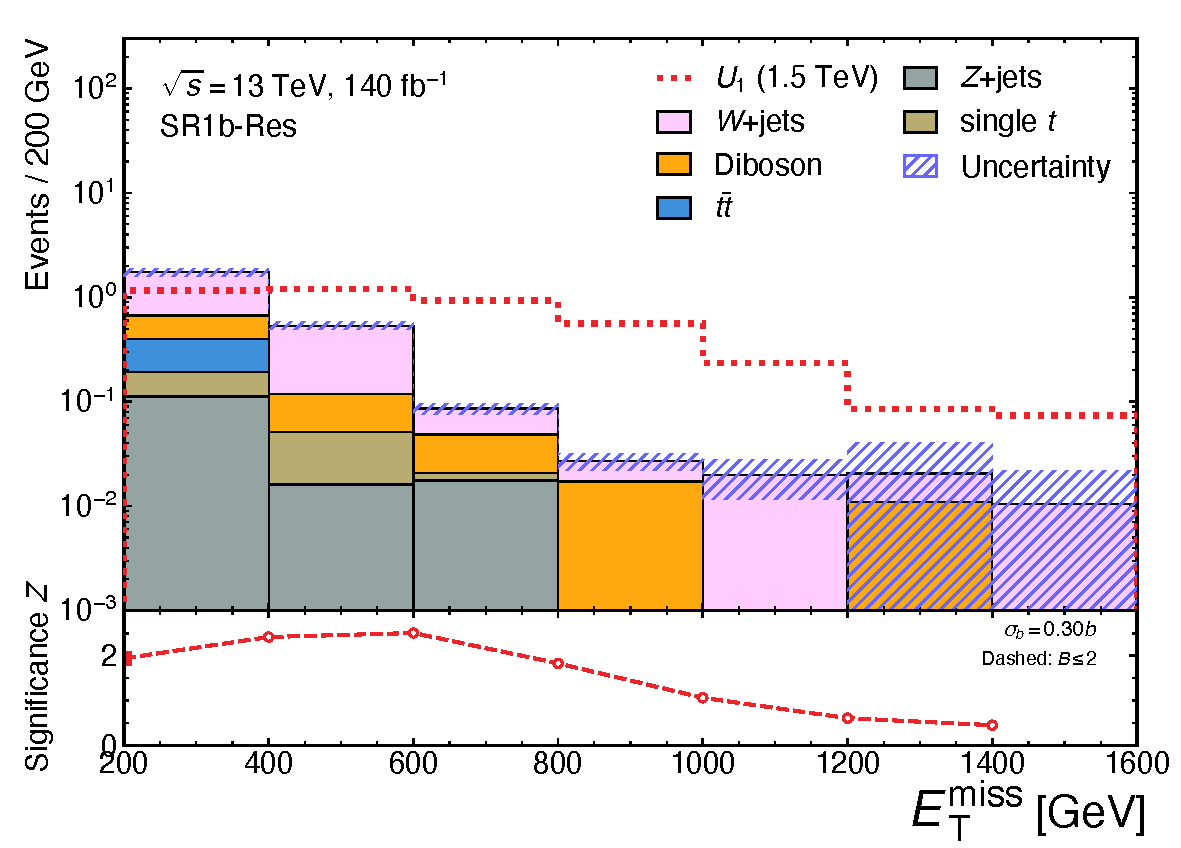
\includegraphics[width=\linewidth]{Figs/CH7/significance/SR1b_Res_met_with_significance.pdf}
        \caption{$\bTagSR$-$\Res$.}
    \end{subfigure}\\[0.5em]
    \begin{subfigure}{0.8\linewidth}
        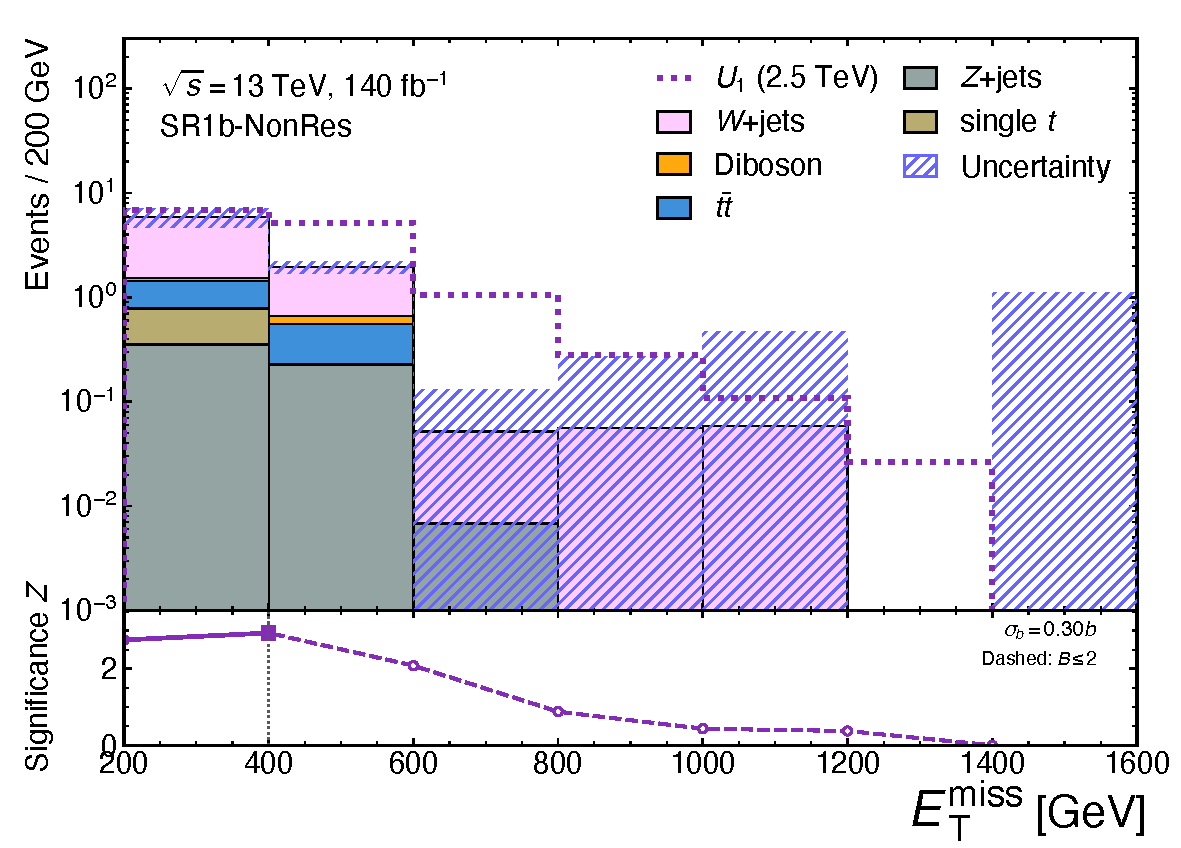
\includegraphics[width=\linewidth]{Figs/CH7/significance/SR1b_NonRes_met_with_significance.pdf}
        \caption{$\bTagSR$-$\NonRes$.}
    \end{subfigure}
    \caption[SR1b missing transverse momentum with significance $Z$]{$N-1$ $\met$ distributions and the corresponding significance $Z$. $Z$ is calculated from the signal and background yields above each threshold, with $\sigma_b=0.30b$. Dashed segments of the $Z$ curves indicate regions where $b\leq2$.}
    \label{fig:ch7_met_with_significance}
\end{figure}

\clearpage
\subsection[SR1b-Res definition]{$\bTagSR$-$\Res$ definition}
\label{subsec:ch7_sr1b_res}

The definition and cutflow for $\bTagSR$-$\Res$ is summarised in Table~\ref{tab:ch7_cutflow_res}, using the resonant optimisation benchmark $(\MU,\gU,\beta_L^{23})=(1.5~\TeV,1.5,0.6)$.
A single event count with $m_{b\tau}>800~\GeV$ is used because the simulated background statistics at high $m_{b\tau}$ are insufficient for a fit to the mass distribution.

\begin{table}[htbp]
    \centering
    \small
    \caption{Signal and background cutflow for $\bTagSR$-$\Res$. The signal is evaluated at $(\MU,\gU,\beta_L^{23})=(1.5~\TeV,1.5,0.6)$. The uncertainties are from MC statistics only.}
    \label{tab:ch7_cutflow_res}
    \setlength{\tabcolsep}{3pt}
    \resizebox{\linewidth}{!}{%
    \begin{tabular}{lrrrrrrr}
        \toprule
        Requirement & Signal & $\ttbar$ & Single top & $W$+jets & $Z$+jets & Diboson & Total background \\
        \midrule
        Baseline & $35.2\pm0.4$ & $1043.0\pm6.9$ & $283.8\pm3.4$ & $2156.9\pm16.1$ & $369.2\pm7.7$ & $173.9\pm2.7$ & $4027.3\pm19.7$ \\
        $\pT^\tau>200~\GeV$ & $19.9\pm0.3$ & $32.3\pm1.3$ & $11.8\pm0.5$ & $108.9\pm9.4$ & $30.4\pm4.7$ & $9.7\pm0.6$ & $193.1\pm10.6$ \\
        $\met>200~\GeV$ & $19.9\pm0.3$ & $32.3\pm1.3$ & $11.8\pm0.5$ & $108.9\pm9.4$ & $30.4\pm4.7$ & $9.7\pm0.6$ & $193.1\pm10.6$ \\
        $\mT>200~\GeV$ & $19.4\pm0.3$ & $25.1\pm1.1$ & $9.2\pm0.4$ & $79.2\pm9.4$ & $24.2\pm4.7$ & $6.9\pm0.5$ & $143.6\pm10.6$ \\
        $m_{b\tau}>800~\GeV$ & $4.9\pm0.1$ & $0.4\pm0.2$ & $0.4\pm0.1$ & $2.8\pm0.4$ & $1.1\pm0.2$ & $0.5\pm0.1$ & $5.2\pm0.5$ \\
        $N_j-N_b\leq3$ & $4.7\pm0.1$ & $0.3\pm0.1$ & $0.2\pm0.1$ & $2.5\pm0.4$ & $0.9\pm0.2$ & $0.4\pm0.1$ & $4.3\pm0.5$ \\
        $\pT^b>250~\GeV$ & $4.2\pm0.1$ & $0.2\pm0.1$ & $0.1\pm0.1$ & $1.5\pm0.2$ & $0.2\pm0.1$ & $0.4\pm0.1$ & $2.4\pm0.3$ \\
        \bottomrule
    \end{tabular}
    }
\end{table}

As a result, the expected signal and background yields are 4.2 and 2.4 events, respectively, giving $Z=1.95$.

The background is dominated by $W(\to\tau\nu)$+jets, which contributes approximately $64\%$.
Approximately $16\%$ is contributed by diboson production.
The top-quark contribution consists of $\ttbar$ ($8\%$) and single-top production ($5\%$), with the latter mainly from the $Wt$ process.
These events are mainly from $\ttbar\to b\tau\nu\,\bar b\tau\nu$ or $Wt\to b\tau\nu\,\tau\nu$ when only one $\tau$ is selected and the other is misidentified as a jet.
A smaller contribution is provided by $Z(\to\tau\tau)$+jets, while the $Z(\to\nu\nu)$+jets contribution is negligibly small.

The $N-1$ distributions in $\bTagSR$-$\Res$ with relaxed kinematic requirements are shown in Figure~\ref{fig:ch7_sr1b_res_distributions}.
To reduce statistical fluctuations, the thresholds on the correlated variables $\mT$ and $\pT^\tau$ are both lowered to $100~\GeV$.

For the $1.5~\TeV$ benchmark, the $m_{b\tau}$ peak is shifted to about $900~\GeV$ because the neutrino from the $\tau$ decay is not included in the reconstructed mass.
The mass distribution is also broadened by the missing neutrino momentum and poor jet reconstruction resolution.

\begin{figure}[htpb]
    \centering
    \begin{subfigure}{0.49\linewidth}
        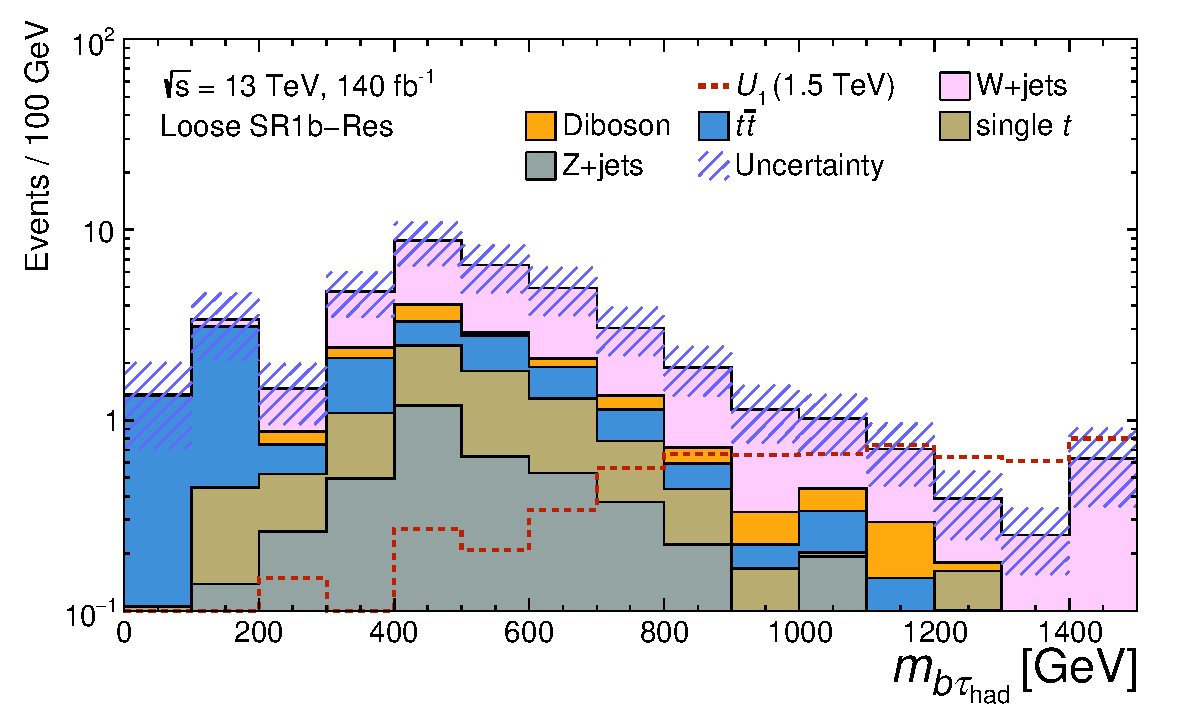
\includegraphics[width=\linewidth]{Figs/CH7/SR1b_Res_InvM.pdf}
        \caption{$m_{b\tau_{\mathrm{had}}}$.}
    \end{subfigure}\hfill
    \begin{subfigure}{0.49\linewidth}
        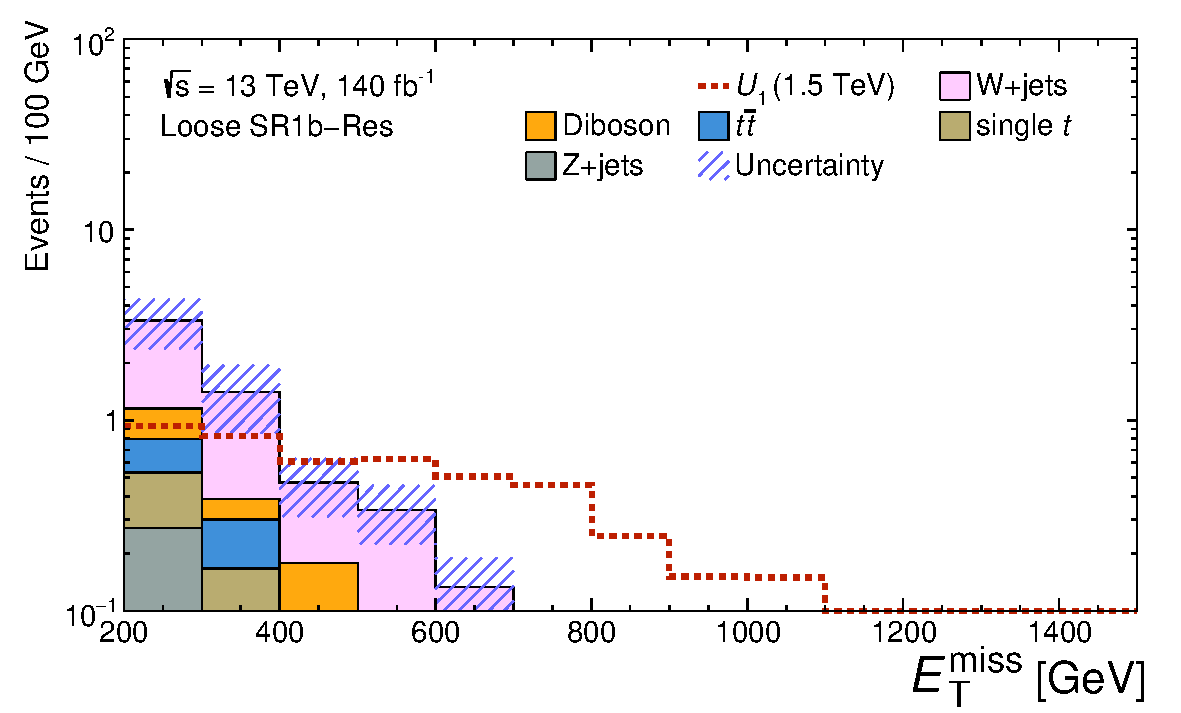
\includegraphics[width=\linewidth]{Figs/CH7/SR1b_Res_met.pdf}
        \caption{$\met$.}
    \end{subfigure}\\
    \begin{subfigure}{0.49\linewidth}
        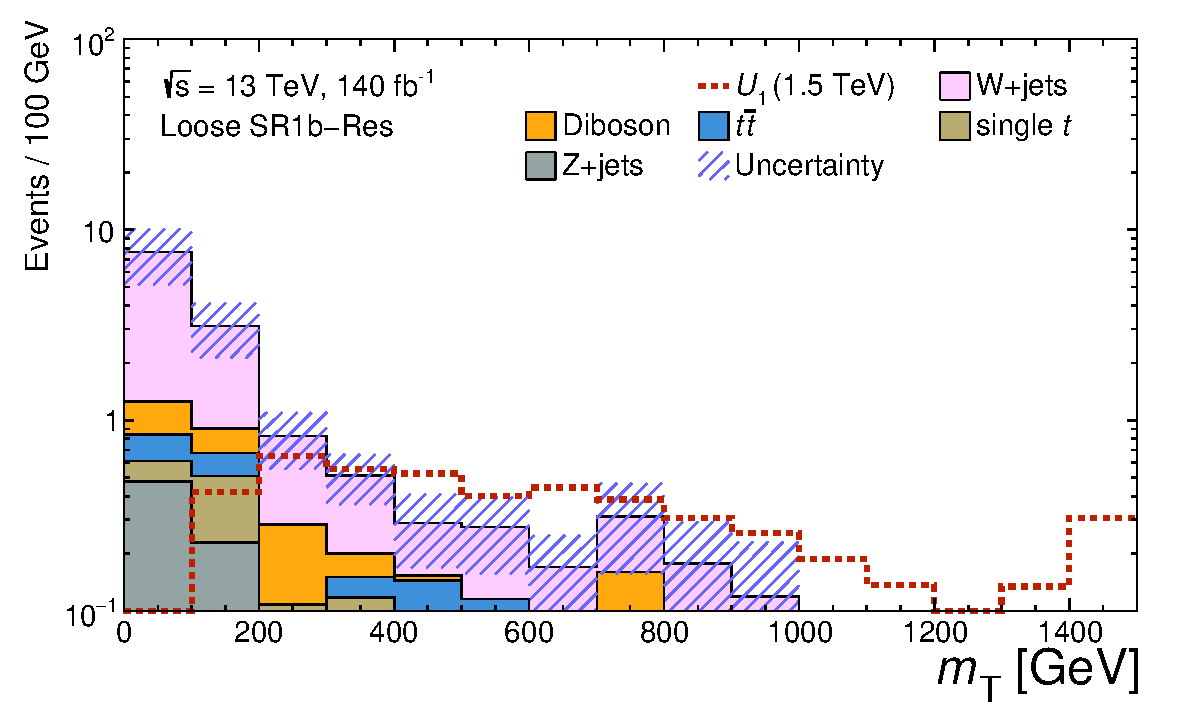
\includegraphics[width=\linewidth]{Figs/CH7/SR1b_Res_mT.pdf}
        \caption{$\mT$.}
    \end{subfigure}\hfill
    \begin{subfigure}{0.49\linewidth}
        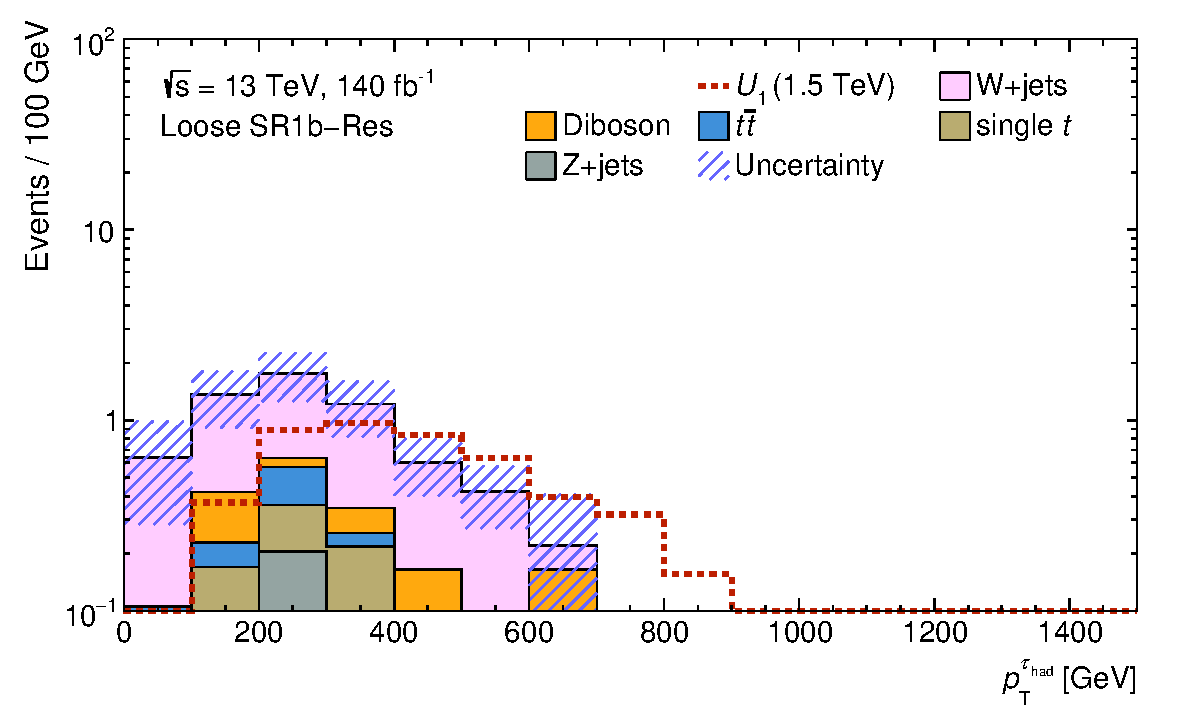
\includegraphics[width=\linewidth]{Figs/CH7/SR1b_Res_tau_pT.pdf}
        \caption{$\pT^{\tau_{\mathrm{had}}}$.}
    \end{subfigure}\\
    \begin{subfigure}{0.49\linewidth}
        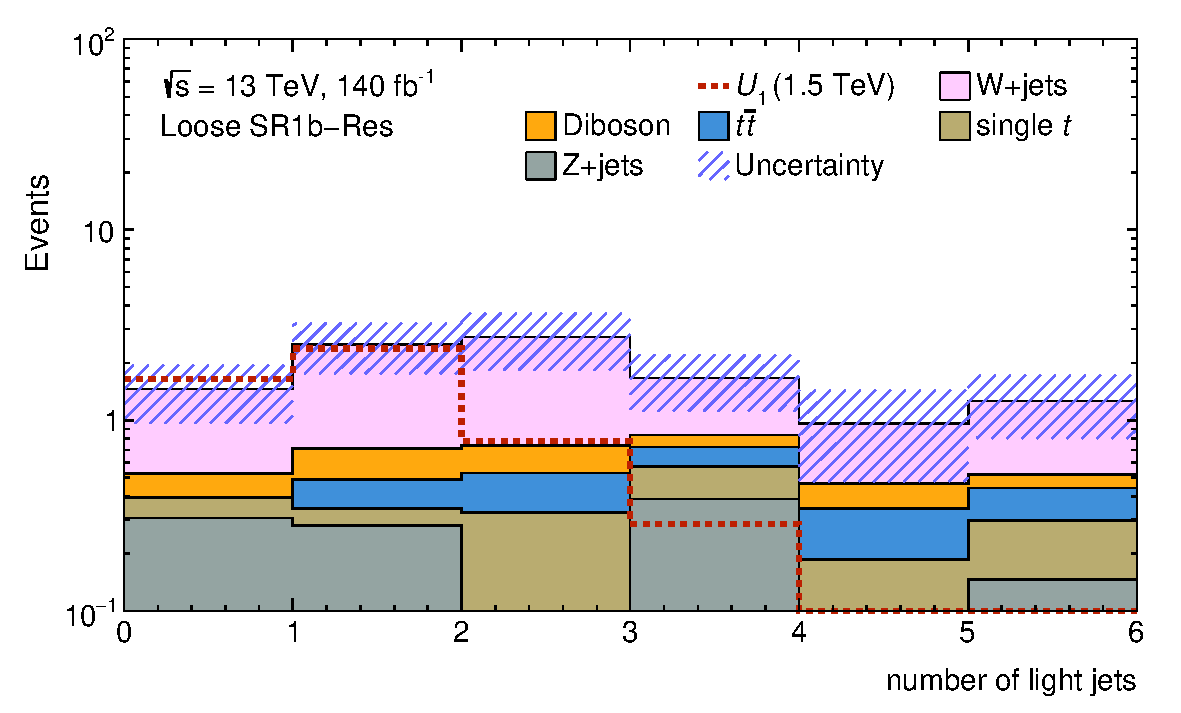
\includegraphics[width=\linewidth]{Figs/CH7/SR1b_Res_nlightjets.pdf}
        \caption{Number of light jets.}
    \end{subfigure}\hfill
    \begin{subfigure}{0.49\linewidth}
        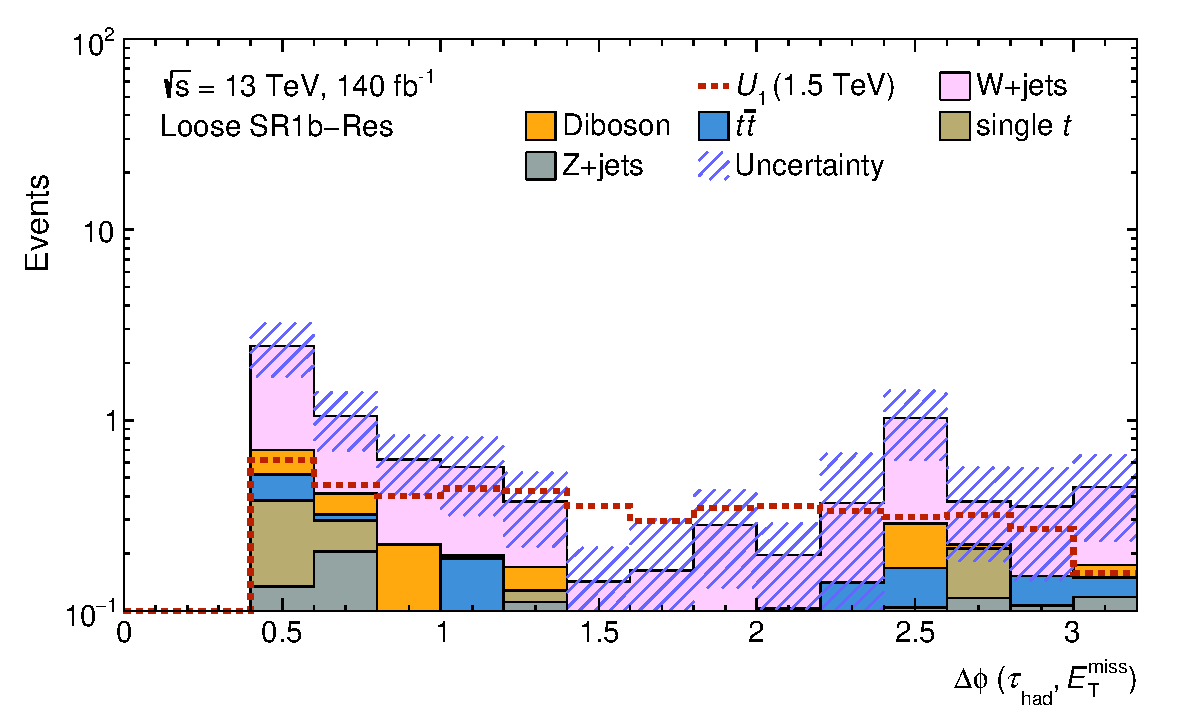
\includegraphics[width=\linewidth]{Figs/CH7/SR1b_Res_dphi.pdf}
        \caption{$\Delta\phi(\tau_{\mathrm{had}},\met)$.}
    \end{subfigure}
    \caption[Loose N-1 distributions in SR1b-Res]{$N-1$ distributions in the loose $\bTagSR$-$\Res$ region. The $\mT$ and $\pT^\tau$ thresholds are reduced to $100~\GeV$. The red dashed line represents the signal at $(\MU,\gU,\beta_L^{23})=(1.5~\TeV,1.5,0.6)$. The hatched band represents the background uncertainty, including systematic contributions. The red arrows mark the final selection thresholds and point towards the retained ranges.}
    \label{fig:ch7_sr1b_res_distributions}
\end{figure}

\clearpage
\subsection[SR1b-NonRes definition]{$\bTagSR$-$\NonRes$ definition}
\label{subsec:ch7_sr1b_nonres}
% 这个section结构模仿上个Section修改
$\bTagSR$-$\NonRes$ is defined by requiring $50<\pT^b<250~\GeV$, $\pT^\tau>200~\GeV$, $\met>400~\GeV$, $\mT>600~\GeV$ and $\DphiTauMet>1.2$, with at most one jet that is not $b$-tagged.
No $m_{b\tau}$ requirement is applied because the $b$-jet and $\tau$ do not reconstruct an on-shell leptoquark in the target topology.
This region also contributes a single event count to the fit.

The background is dominated by $W$+jets, principally $W\to\tau\nu$, which contributes approximately $69\%$.
The next-largest contribution is from $\ttbar$ ($16\%$), followed by $Z\to\tau\tau$+jets ($8\%$) and diboson production ($5\%$).
The $Z\to\tau\tau$ contribution requires only one selected $\tau$, with neutrinos from the decays producing $\met$.
In both $\bTagSR$ regions, $Z\to\nu\nu$+jets is the main source of events with a jet misidentified as a $\tau$, because the invisible $Z$ decay supplies the missing momentum.
Multijet production is negligible after the cleaning and full SR requirements.

For the optimisation benchmark $(\MU,\gU,\beta_L^{23})=(2.5~\TeV,2.5,1.0)$, the expected signal and background yields are 6.583 and 2.097 events, respectively, giving $Z=2.94$.

\begin{table}[htbp]
    \centering
    \small
    \caption{Signal ($S$) and background ($B$) cutflow in the $\bTagSR$-$\NonRes$ optimisation for $(\MU,\gU,\beta_L^{23})=(2.5~\TeV,2.5,1.0)$.}
    \label{tab:ch7_cutflow_nonres}
    \begin{tabular}{lrr}
        \toprule
        Cumulative requirement & $S$ & $B$ \\
        \midrule
        Baseline & 111.0 & 4027.3 \\
        $\pT^\tau>200~\GeV$ & 70.5 & 193.1 \\
        $\met>400~\GeV$ & 26.4 & 15.1 \\
        $\mT>600~\GeV$ & 24.0 & 6.4 \\
        $\DphiTauMet>1.2$ & 23.8 & 6.4 \\
        $N_j-N_b\leq1$ & 17.2 & 2.8 \\
        $50<\pT^b<250~\GeV$ & 6.6 & 2.1 \\
        \bottomrule
    \end{tabular}
\end{table}

The yields and significances for both regions are summarised in Table~\ref{tab:ch7_prefit_yields}.
The yields agree with the rounded endpoints of the optimisation cutflows to within $2\%$.
The cutflows describe the optimisation study, while the final selections are chosen with the statistical uncertainty in the background prediction kept below $30\%$.

\begin{table}[htbp]
    \centering
    \small
    \caption{Signal and background yields for the two optimisation benchmarks in the final $\bTagSR$ selections. The approximate significance is evaluated with $\sigma_b=0.30b$.}
    \label{tab:ch7_prefit_yields}
    \begin{tabular}{lcrrr}
        \toprule
        SR & $(\MU,\gU,\beta_L^{23})$ & $S$ & $B$ & $Z$ \\
        \midrule
        $\bTagSR$-$\Res$ & $(1.5~\TeV,1.5,0.6)$ & 4.262 & 2.439 & 1.95 \\
        $\bTagSR$-$\NonRes$ & $(2.5~\TeV,2.5,1.0)$ & 6.583 & 2.097 & 2.94 \\
        \bottomrule
    \end{tabular}
\end{table}

The loose $N-1$ distributions in Figure~\ref{fig:ch7_sr1b_nonres_distributions} illustrate the high-$\mT$ and high-$\met$ tails of the non-resonant signal.
The $\mT$, $\met$ and $\pT^\tau$ thresholds are each lowered by $100~\GeV$ before the plotted requirement is removed.
The trigger-plateau requirement $\met>200~\GeV$ is retained.

\begin{figure}[htpb]
    \centering
    \begin{subfigure}{0.49\linewidth}
        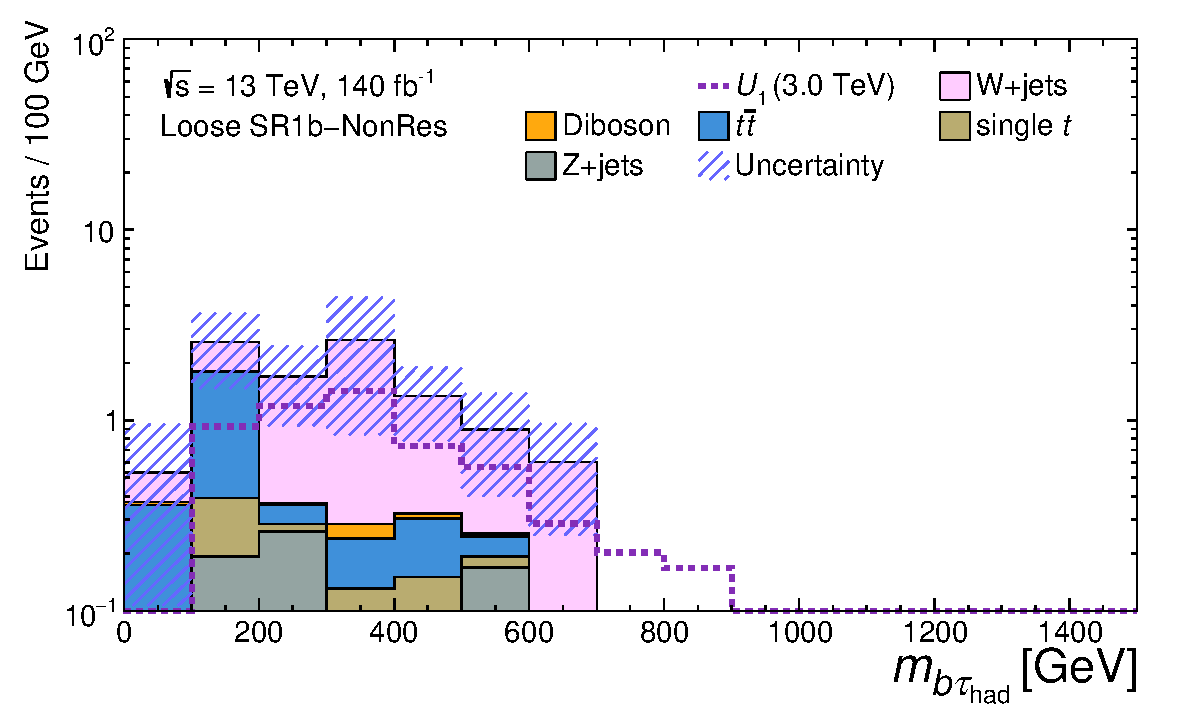
\includegraphics[width=\linewidth]{Figs/CH7/SR1b_NonRes_InvM.pdf}
        \caption{$m_{b\tau_{\mathrm{had}}}$.}
    \end{subfigure}\hfill
    \begin{subfigure}{0.49\linewidth}
        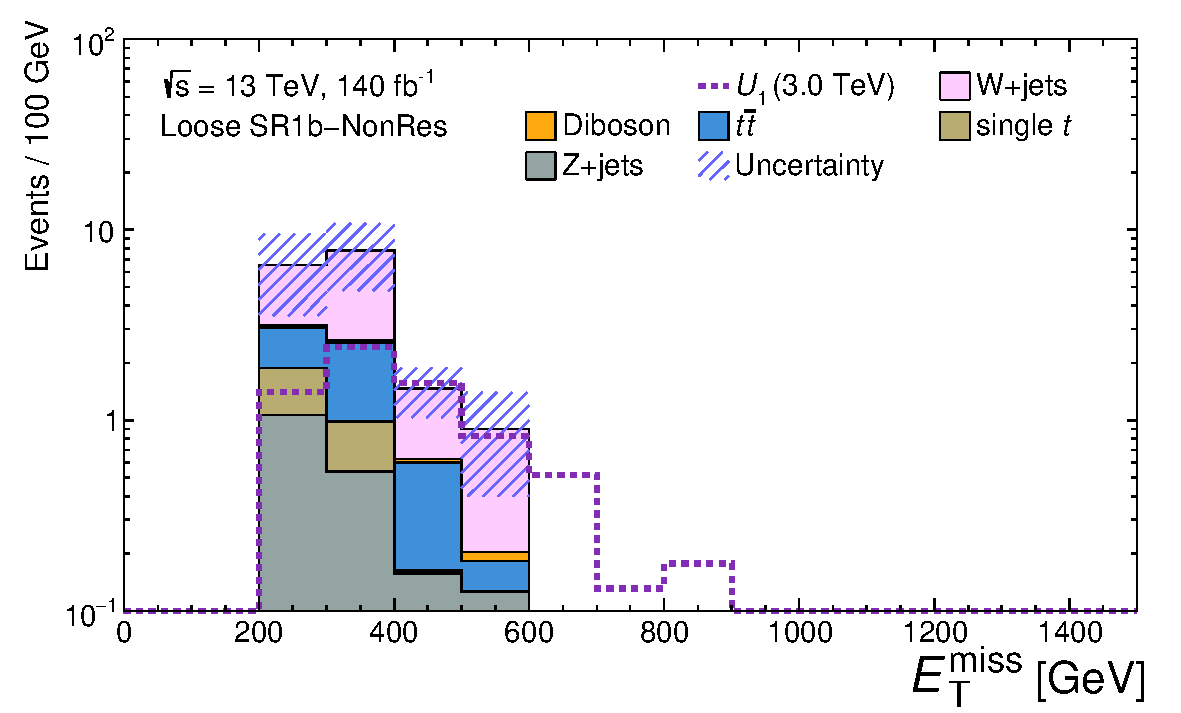
\includegraphics[width=\linewidth]{Figs/CH7/SR1b_NonRes_met.pdf}
        \caption{$\met$.}
    \end{subfigure}\\
    \begin{subfigure}{0.49\linewidth}
        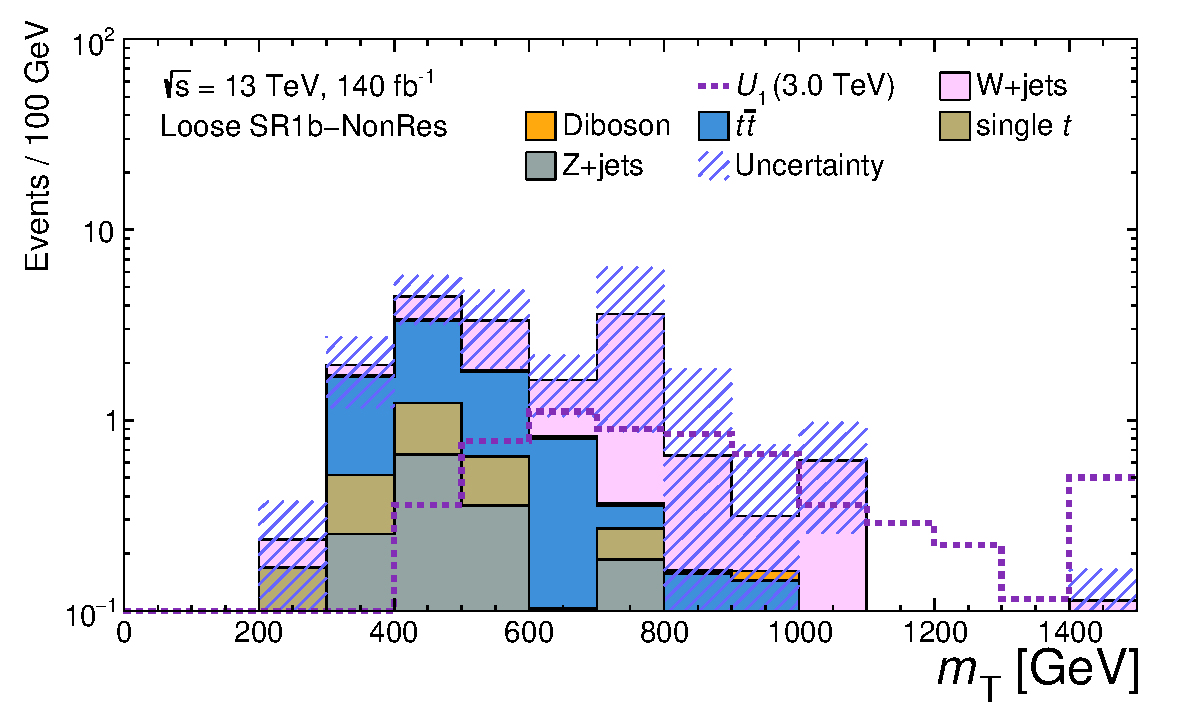
\includegraphics[width=\linewidth]{Figs/CH7/SR1b_NonRes_mT.pdf}
        \caption{$\mT$.}
    \end{subfigure}\hfill
    \begin{subfigure}{0.49\linewidth}
        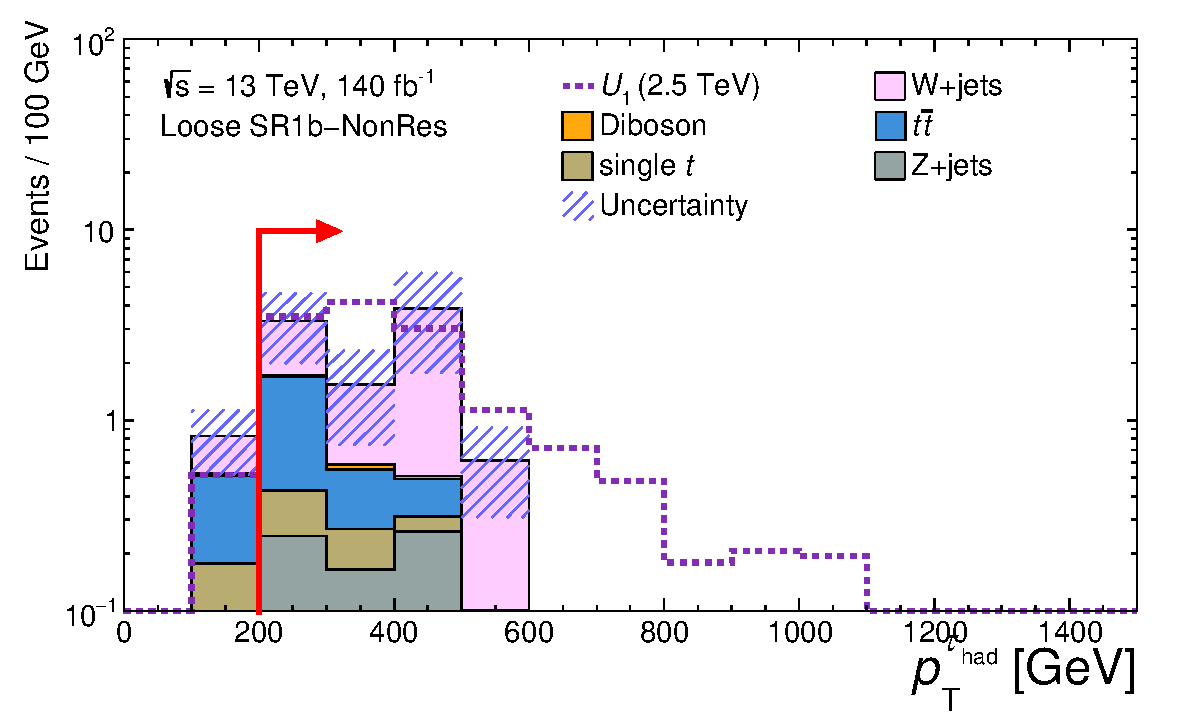
\includegraphics[width=\linewidth]{Figs/CH7/SR1b_NonRes_tau_pT.pdf}
        \caption{$\pT^{\tau_{\mathrm{had}}}$.}
    \end{subfigure}\\
    \begin{subfigure}{0.49\linewidth}
        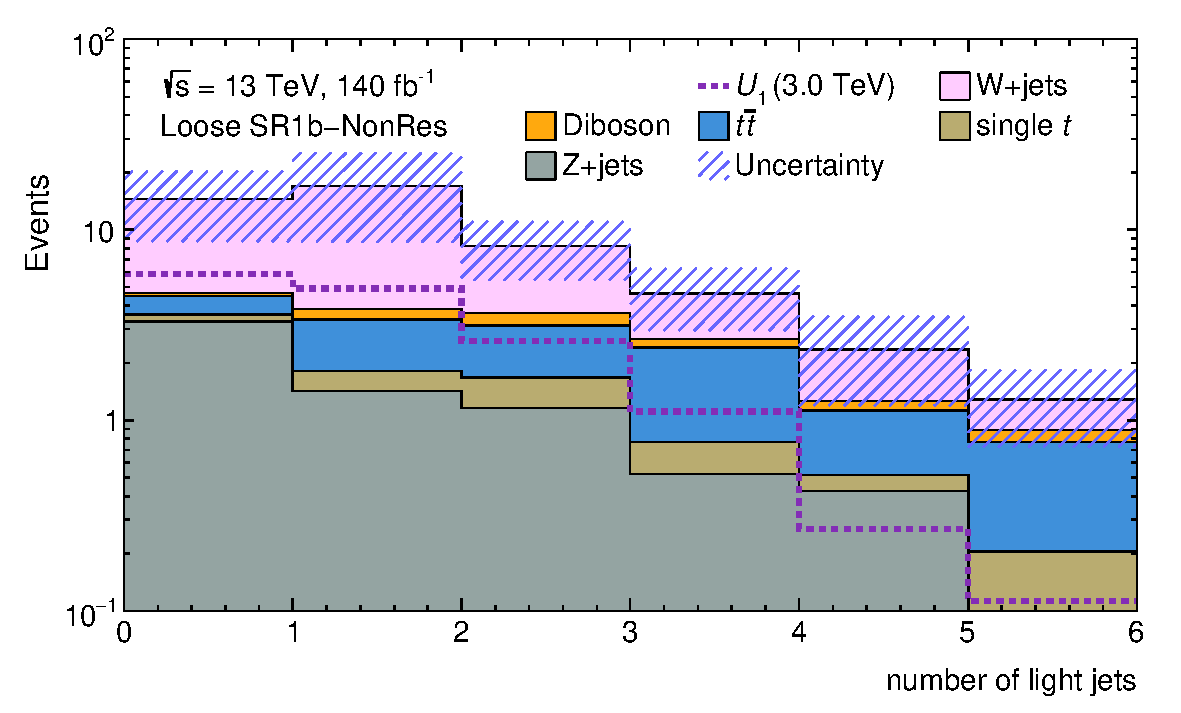
\includegraphics[width=\linewidth]{Figs/CH7/SR1b_NonRes_nlightjets.pdf}
        \caption{Number of light jets.}
    \end{subfigure}\hfill
    \begin{subfigure}{0.49\linewidth}
        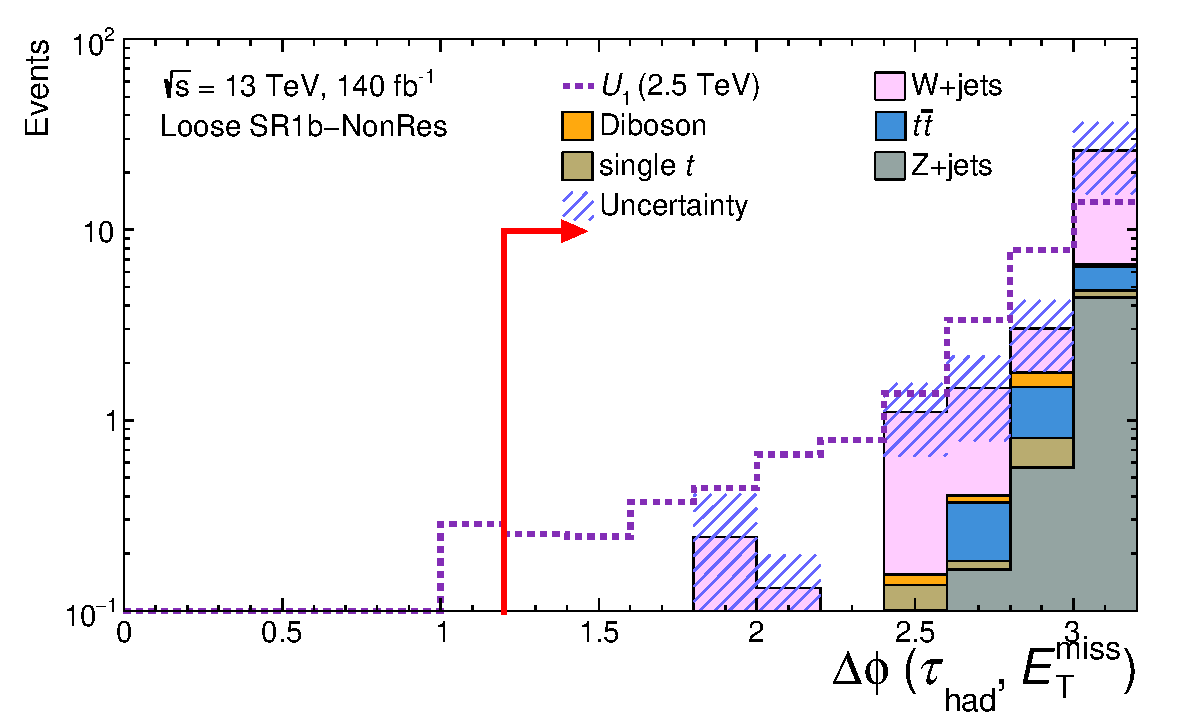
\includegraphics[width=\linewidth]{Figs/CH7/SR1b_NonRes_dphi.pdf}
        \caption{$\Delta\phi(\tau_{\mathrm{had}},\met)$.}
    \end{subfigure}
    \caption[Loose N-1 distributions in SR1b-NonRes]{$N-1$ distributions in the loose $\bTagSR$-$\NonRes$ region. The thresholds are lowered to $\mT>500~\GeV$, $\met>300~\GeV$ and $\pT^\tau>100~\GeV$. The baseline $\met>200~\GeV$ is retained. The hatched band represents the background uncertainty, including systematic contributions. The purple dashed line represents the signal at $(\MU,\gU,\beta_L^{23})=(3.0~\TeV,2.5,1.0)$. The red arrows mark the final selection thresholds and point towards the retained ranges.}
    \label{fig:ch7_sr1b_nonres_distributions}
\end{figure}

\clearpage
\section[b-veto signal region definition (SR0b)]{b-veto signal region definition ($\bVetoSR$)}
\label{sec:ch7_sr0b}

The $\bVetoSR$ regions is defined based on the $\bTagSR$ optimisation results, focusing on extracting the on-shell $s\tau$ instead of $b\tau$ LQ decays to extend the sensitivity to large $\beta_L^{23}$.
The corresponding signal topologys were introduced in Section~\ref{subsec:lq_collider_benchmark}.
In particular, $U_1\to s\tau$ produces a resonant signal with a genuine non-$b$ jet, so $\bVetoSR$ retains a physically distinct signal contribution in addition to events in which a $b$-jet is not tagged or reconstructed.
The leading jet in $\bVetoSR$ is not explicitly identified as a strange-quark jet.
The truth-level study also identifies a substantial contribution with a leading $c$ jet.
At $(\MU,\gU,\beta_L^{23})=(1.5~\TeV,1.5,0.6)$, approximately $30\%$ and $60\%$ of the selected truth-level resonant-category events have a leading $s$ or $c$ jet, respectively.
The $s$-jet contribution contains the $s\tau$ resonance, whereas the $c$-jet contribution can contain an on-shell $U_1\to c\nu_\tau$ decay.
For the latter, the resonance is in the $c\nu_\tau$ system rather than the jet--$\tau$ system.
In the non-resonant truth-level category, approximately $33\%$ and $11\%$ of the events have a radiated leading $s$ or $c$ jet, with most of the remainder containing a gluon jet in $sc\to\tau\nu_\tau$ production.
These fractions describe the chosen benchmark and truth selection, rather than a flavour measurement of the reconstructed jets.

The two $\bVetoSR$ regions are defined by replacing the one-$b$-jet requirement with $N_b=0$ and using the leading jet in the topology-dependent selections.
The resonant region requires $\pT^{j_1}>250~\GeV$ and $m_{j\tau}>800~\GeV$, while the non-resonant region requires $50<\pT^{j_1}<250~\GeV$.
The $\pT^\tau$, $\met$, $\mT$ and $\DphiTauMet$ thresholds follow the corresponding one-$b$-jet regions.
The upper limits are imposed on the total jet multiplicity: $N_j\leq4$ for $\bVetoSR$-$\Res$ and $N_j\leq2$ for $\bVetoSR$-$\NonRes$.
These preserve the total jet limits used in $\bTagSR$ after replacing the tagged jet with an untagged leading jet.

The $\met>200~\GeV$ requirement in $\bVetoSR$-$\Res$ is retained to keep its kinematic selection aligned with $\bTagSR$-$\Res$.
A supplementary study of tighter $\met$ thresholds is presented in Appendix~\ref{app:sr0b_optimisation}.
The $\bVetoSR$-$\NonRes$ threshold remains $\met>400~\GeV$, which also maximises the significance in that study.

The destructive interference in the final zero-$b$-jet selections reduces the nominal pure BSM yield by approximately $20\%$ at $\MU=1.5~\TeV$ and by about $30$--$40\%$ at higher masses.
This reduction is appreciable even after the high-$\mT$ and $\met$ requirements, so the final prediction includes the signed interference contribution explicitly.
The supplementary $\met$ scan in Appendix~\ref{app:sr0b_optimisation} also shows that a higher $\met$ threshold can suppress this contribution.

Figure~\ref{fig:ch7_sr0b_distributions} shows the $m_{j\tau}$ distribution before the mass requirement in $\bVetoSR$-$\Res$.
It also shows the transverse-mass distribution above $600~\GeV$ in $\bVetoSR$-$\NonRes$.
The high-$m_{j\tau}$ requirement enhances the resonant signal contribution, while the high-$\mT$ requirement selects non-resonant production.
Together with the one-$b$-jet regions, these selections retain sensitivity to both $b\tau$ and $s\tau$ final states over the coupling range studied in this thesis.

\begin{figure}[htpb]
    \centering
    \begin{subfigure}{0.49\linewidth}
        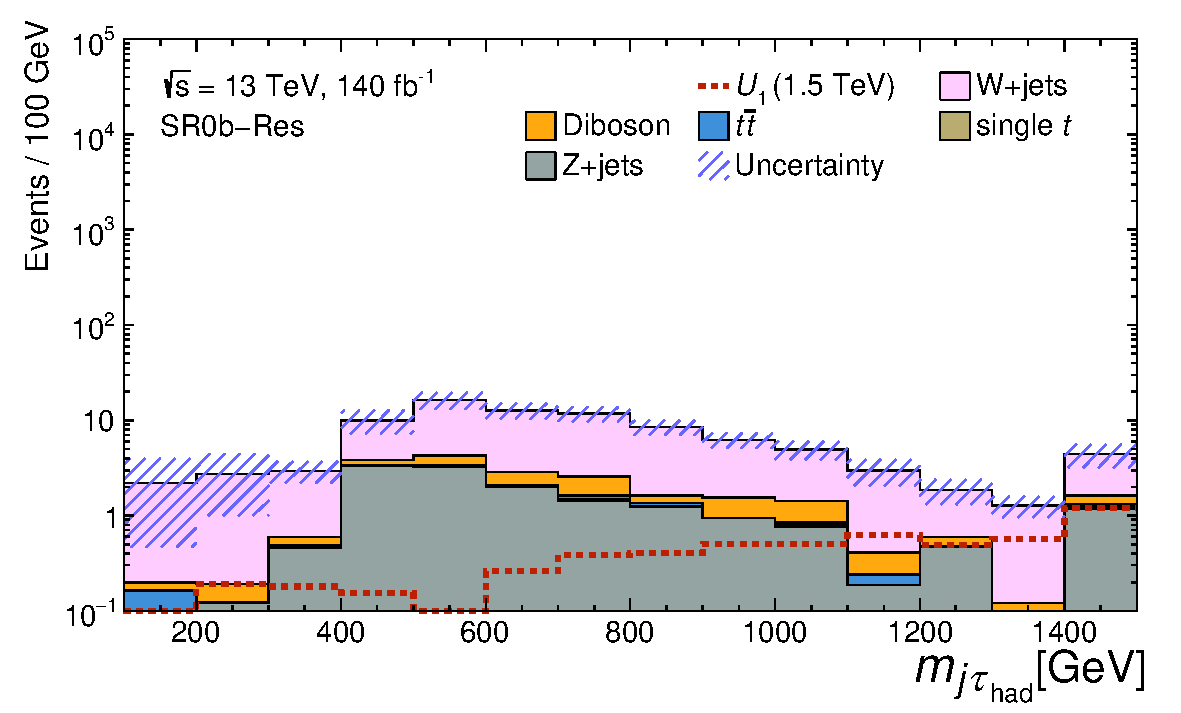
\includegraphics[width=\linewidth]{Figs/CH7/SR0b_Res_InvM.pdf}
        \caption{$\bVetoSR$-$\Res$: $m_{j\tau}$.}
    \end{subfigure}\hfill
    \begin{subfigure}{0.49\linewidth}
        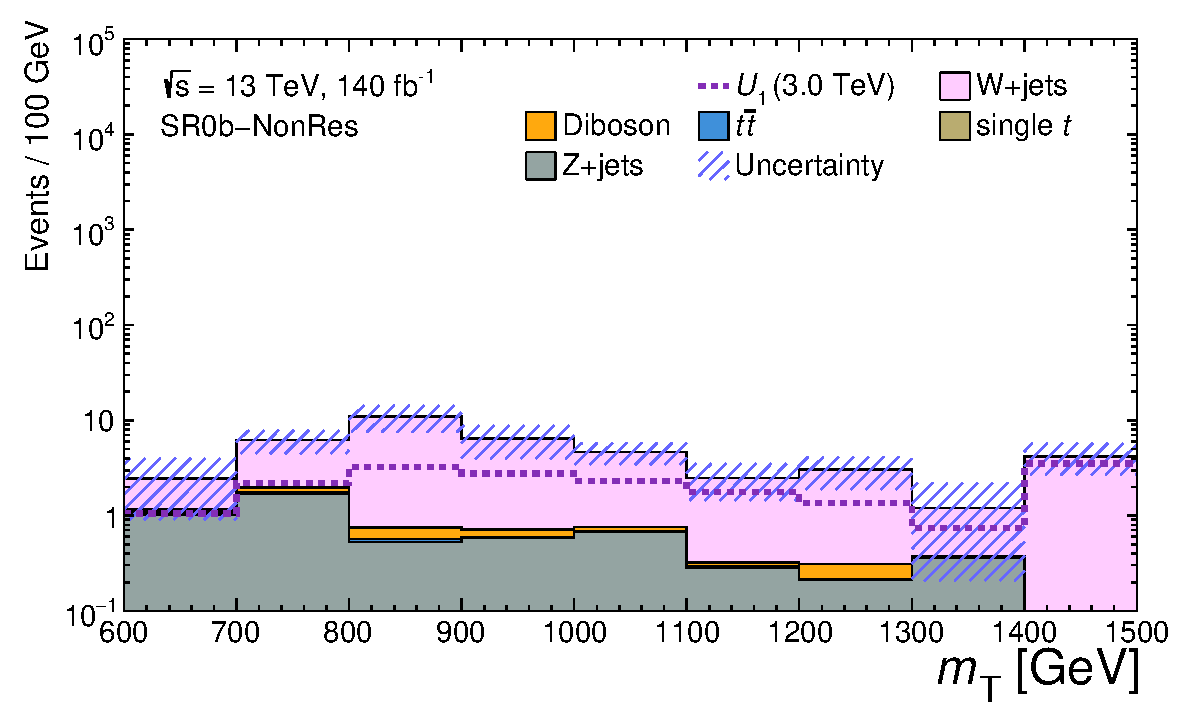
\includegraphics[width=\linewidth]{Figs/CH7/SR0b_NonRes_mT.pdf}
        \caption{$\bVetoSR$-$\NonRes$: $\mT$.}
    \end{subfigure}
    \caption[Discriminating-variable distributions in SR0b]{Distributions of (a) $m_{j\tau}$ in $\bVetoSR$-$\Res$ with the mass requirement removed and (b) $\mT$ in $\bVetoSR$-$\NonRes$ above $600~\GeV$. The other SR requirements are retained. The hatched band represents the background uncertainty. The dotted curves show pure BSM signals at $(\MU,\gU,\beta_L^{23})=(1.5~\TeV,1.5,0.6)$ in (a) and $(3.0~\TeV,2.5,1.0)$ in (b).}
    \label{fig:ch7_sr0b_distributions}
\end{figure}

The zero-$b$-jet background is dominated by $W\to\tau\nu$+jets, since vetoing tagged $b$ jets removes much of the top-quark background while retaining $W$ production with light-flavour jets.
In the final prediction after the control-region constraints, $W$+jets contributes approximately $76\%$ in $\bVetoSR$-$\Res$ and $82\%$ in $\bVetoSR$-$\NonRes$.
In the resonant region, diboson production contributes about $10\%$, $Z\to\nu\nu$+jets about $8\%$, and $Z\to\tau\tau$+jets about $5\%$.
In the non-resonant region, the corresponding contributions are approximately $3\%$, $6\%$ and $8\%$.
The $Z\to\nu\nu$ events contain a jet misidentified as a $\tau$, while $Z\to\tau\tau$ and diboson events can contain genuine $\tau$ leptons and neutrinos.
The top-quark background contribution is below $1\%$ in each zero-$b$-jet region.

The final requirements for all four mutually exclusive SRs are summarised in Table~\ref{tab:ch7_signal_regions}.
Each region contributes one event count to the simultaneous statistical analysis.

\begin{table}[htbp]
    \centering
    \small
    \caption{Common baseline requirements and final signal-region selections. A dash denotes no additional requirement. The jet multiplicity includes $b$-tagged jets.}
    \label{tab:ch7_signal_regions}
    \begin{tabular}{lcccc}
        \toprule
        \multicolumn{5}{c}{Baseline requirements} \\
        \midrule
        Trigger & \multicolumn{4}{c}{Lowest-threshold unprescaled $\met$ trigger} \\
        $N_\tau$ & \multicolumn{4}{c}{1} \\
        $N_\ell=N_e+N_\mu$ & \multicolumn{4}{c}{0} \\
        Multijet suppression & \multicolumn{4}{c}{$\minDphiJetMet>0.4$ or $\metOverMinDphiJetPt>6$} \\
        \midrule
        & \multicolumn{2}{c}{Resonant} & \multicolumn{2}{c}{Non-resonant} \\
        Requirement & $\bTagSR$-$\Res$ & $\bVetoSR$-$\Res$ & $\bTagSR$-$\NonRes$ & $\bVetoSR$-$\NonRes$ \\
        \midrule
        $N_b$ & 1 & 0 & 1 & 0 \\
        $\pT^b$ [$\GeV$] & $>250$ & -- & $50<\pT^b<250$ & -- \\
        $\pT^{j_1}$ [$\GeV$] & -- & $>250$ & -- & $50<\pT^{j_1}<250$ \\
        $\pT^\tau$ [$\GeV$] & \multicolumn{4}{c}{$>200$} \\
        $\met$ [$\GeV$] & \multicolumn{2}{c}{$>200$} & \multicolumn{2}{c}{$>400$} \\
        $\mT$ [$\GeV$] & \multicolumn{2}{c}{$>200$} & \multicolumn{2}{c}{$>600$} \\
        $m_{b\tau}$ [$\GeV$] & $>800$ & -- & -- & -- \\
        $m_{j\tau}$ [$\GeV$] & -- & $>800$ & -- & -- \\
        $\DphiTauMet$ & \multicolumn{2}{c}{--} & \multicolumn{2}{c}{$>1.2$} \\
        $N_j$ & \multicolumn{2}{c}{$\leq4$} & \multicolumn{2}{c}{$\leq2$} \\
        \bottomrule
    \end{tabular}
\end{table}

\clearpage
\section{Tau-pair signal contamination}
\label{sec:ch7_tautau_contamination}

Leptoquark production with a $\tau\tau$ final state can also populate the $\tau\nu+\mathrm{jets}$ signal regions.
Although two $\tau$-leptons are produced, an event can satisfy the single-$\tau$ requirement when only one is reconstructed and selected.
Neutrinos from the $\tau$ decays produce missing momentum.
This is an additional BSM contribution from the same $U_1$ model, rather than an SM background.

The study uses simulated $\tau\tau$ samples generated with $\beta_L^{33}=1$, $\beta_R^{33}=0$ and $\beta_L^{23}=0$.
Their selected yields are compared with available $\tau\nu$ samples near the exclusion sensitivity, at $(\MU,\gU,\beta_L^{23})=(1.8~\TeV,3.0,0.6)$ and $(3.0~\TeV,2.0,1.4)$.
The corresponding $\tau\tau$ samples use $\gU=2.8$ and $2.1$.
The $\tau\tau$ production cross section is recalculated with \textsc{MadGraph5\_aMC@NLO} at larger $\beta_L^{23}$, and the selected yields are scaled by the cross-section ratio to their generation point.
This estimates the additional rate while retaining the acceptance and kinematic shapes of the available samples.
It therefore provides a sensitivity study rather than a simulation of the full coupling dependence of the $\tau\tau$ acceptance.

The estimated additional yield is of order $35\%$ of the nominal $\tau\nu$ yield in the one-$b$-jet regions and several percent in the zero-$b$-jet regions.
To assess the effect on the search, the nominal signal predictions are increased by the factors shown in Table~\ref{tab:ch7_tautau_contamination}, and the exclusion fit is repeated.

\begin{table}[htbp]
    \centering
    \caption{Additional signal normalisation used to estimate the sensitivity to $\tau\tau$ production. The factors multiply the nominal $\tau\nu$ signal prediction in the supplementary fit.}
    \label{tab:ch7_tautau_contamination}
    \begin{tabular}{lcc}
        \toprule
        Region & Additional contribution & Applied factor \\
        \midrule
        $\bTagSR$-$\Res$ & $37\%$ & 1.37 \\
        $\bTagSR$-$\NonRes$ & $33\%$ & 1.33 \\
        $\bVetoSR$-$\Res$ & $5\%$ & 1.05 \\
        $\bVetoSR$-$\NonRes$ & $7\%$ & 1.07 \\
        \bottomrule
    \end{tabular}
\end{table}

The expected upper limit on the signal strength improves by approximately $8$--$14\%$ in this test.
The corresponding change in the coupling limit is smaller because the signal rate depends strongly on $\gU$.
At $\MU=1.8~\TeV$ and $\beta_L^{23}=0.6$, the expected upper limit on $\gU$ changes from 2.18 to 2.07, an improvement of approximately $5\%$.
At $\MU=3.0~\TeV$ and $\beta_L^{23}=1.4$, it changes from 1.96 to 1.91, or approximately $2.6\%$.
The nominal interpretation retains the $\tau\nu$ signal model.
The supplementary study indicates that the omitted positive $\tau\tau$ contribution could strengthen the expected coupling constraints by a few percent under the assumptions used for the rate estimate.
